\section{Simulation and Data Sample}

The method by which all of the measurements presented in this thesis are done is that of \emph{Monte-Carlo (MC) forward folding}. In a nutshell, this method involves producing a large set of simulated data and background events that are then re-weighted in such a way that their distribution matches that of the observed data events as closely as possible. In order to give accurate results, an accurate simulation of all the particle interactions described in section~\ref{sec:particle-interactions} as well as the detector electronics described in section~\ref{sec:dom-daq} is required. Both simulated and observed events are then passed through the same data processing chain described in section~\ref{sec:data-processing}. The resulting MC simulated dataset and the observed dataset are then histogrammed in the same binning, and the weights of the MC events are adjusted to give the best match between the histograms according to a loss function as defined in section~\ref{sec:test-statistic}.

\subsection{Simulation of Particle Interactions}

\subsection{Simulation of Detector Response}

\subsection{Final Sample and Binning}
\label{sec:sample-binning}
The starting point for this analysis is a DeepCore data sample consisting of 7.5 years of good live time and 21,914 events that pass through all selection steps described in section~\ref{sec:data-processing}. For every event in the sample, the energy and zenith angle is reconstructed as discussed in section~\ref{sec:event-reconstruction}. Both data and simulation sets are binned in reconstructed energy ($E_{\rm reco}$), cosine of the reconstructed zenith angle ($\cos(\theta_z)$), and PID as follows:

\begin{itemize}
    \item $E_{\rm reco}$: 11 bins spanning the range from 6.31~GeV to 158.49~GeV, the two bins with the highest energy are merged.
    \item $\cos(\theta_z)$: 10 bins spanning the range from -1 to 0.1
    \item PID: One bin between 0.55 and 0.75, and one bin between 0.75 and 1.0.
\end{itemize}

The lower PID bin between 0.55 and 0.75 consists to 69\%  (pre-fit MC estimate) of charged-current $\nu_\mu + \bar{\nu}_\mu$ events and is referred to as the \emph{mixed} channel, while the higher PID channel between 0.75 and 1.0 consists to 94\% of charged-current $\nu_\mu + \bar{\nu}_\mu$ events and is referred to as the \emph{tracks} channel. The histogram of both channels at the null hypothesis (i.e. no sterile signal) is shown in figure~\ref{fig:nominal-hist-null-hypo}.

\begin{figure}
    \centering
    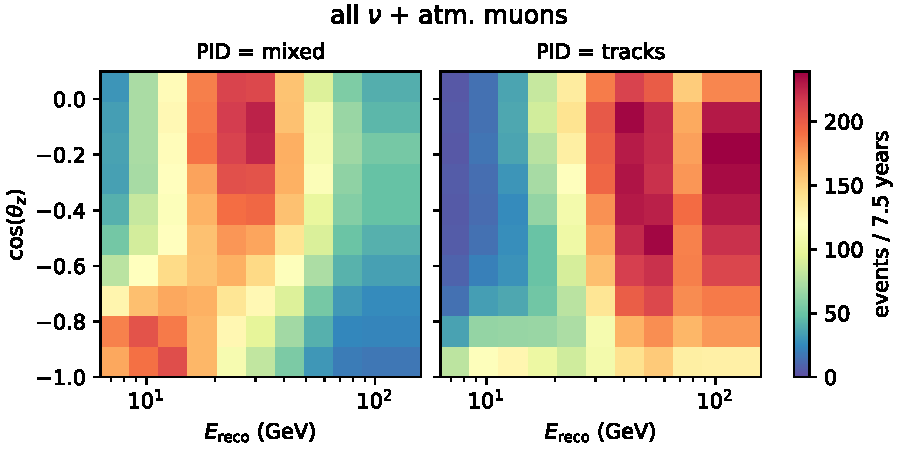
\includegraphics[width=0.8\textwidth]{figures/measurement/simulation_and_data/binning/plot_maps_total.pdf}
    \caption{Expected event counts in 7.5 years of live time assuming no sterile mixing and NuFit~4.0~\cite{nufit40} global best fit parameters at Normal Ordering.}
    \label{fig:nominal-hist-null-hypo}
\end{figure}

\begin{table}[htb]
\centering
\caption{Expected event rate with 8 years livetime broken down in event types and PID bins, calculated at NuFit~4.0 global best fit parameters.}
\label{tab:event-rate}
\begin{tabular}{lccc} \toprule
\hline
Type  & PID & Counts [8 years] & Rate [$\mathrm{\mu Hz}$] \\ \hline
All MC & mixed  &   11428 &   48.3\\
All MC & tracks &   12238 &   51.7\\ \hline
${\nu_{\rm all}} + {\bar\nu_{\rm all}} \, {\rm NC} $ & mixed  &     943 &    4.0 \\
${\nu_e} + {\bar\nu_e} \, {\rm CC}                 $ & mixed  &    1704 &    7.2 \\
${\nu_\mu} + {\bar\nu_\mu} \, {\rm CC}             $ & mixed  &    7901 &   33.4 \\
${\nu_\tau} + {\bar\nu_\tau} \, {\rm CC}           $ & mixed  &     470 &    2.0 \\
muons                                                & mixed  &     410 &    1.7 \\
\hline
${\nu_{\rm all}} + {\bar\nu_{\rm all}} \, {\rm NC} $ & tracks &     171 &    0.7 \\
${\nu_e} + {\bar\nu_e} \, {\rm CC}                 $ & tracks &     294 &    1.2 \\
${\nu_\mu} + {\bar\nu_\mu} \, {\rm CC}             $ & tracks &   11517 &   48.7 \\
${\nu_\tau} + {\bar\nu_\tau} \, {\rm CC}           $ & tracks &     162 &    0.7 \\
muons                                                & tracks &      93 &    0.4 \\
\hline
\hline
\end{tabular}
\end{table}
